\documentclass[11pt,twoside,english,singlespacing,headsepline,consistentlayout]{auxiliary/si-msc-thesis}

\usepackage[utf8]{inputenc} % Required for inputting international characters
\usepackage[T1]{fontenc} % Output font encoding for international characters

\usepackage{lipsum}
\usepackage{mathpazo}
\usepackage{setspace}

\usepackage{lipsum}
\usepackage{float}
\usepackage{listings}
\usepackage{wrapfig}
\usepackage{algorithm}
\usepackage{algpseudocode}
\usepackage{subcaption}
\usepackage{graphicx}
\usepackage{csquotes}

\def\sectionautorefname{Section}
\def\subsectionautorefname{Subsection}

\usepackage{tikz}

\newcommand\encircle[1]{%
  \tikz[baseline=(X.base)] 
    \node (X) [draw, shape=circle, inner sep=0] {\strut #1};}

\lstdefinelanguage{algebra}
{morekeywords={import,sort,constructors,observers,transformers,axioms,if,
else,end},
sensitive=false,
morecomment=[l]{//s},
}

\newcommand{\quotes}[1]{``#1''}

\usepackage{listings}
\lstloadlanguages{Ruby}



%%%%%%%%%%%%%%%%%%%%%%%%%%%%%%%%%%%%%%%%%%%%%%%%%%%%%%%%%%%%%%%%%
%%%	MARGIN SETTINGS %%%%%%%%%%%%%%%%%%%%%%%%%%%%%%%%%%%%%%%%%%%%%
%%%%%%%%%%%%%%%%%%%%%%%%%%%%%%%%%%%%%%%%%%%%%%%%%%%%%%%%%%%%%%%%%

\geometry{paper=a4paper, inner=1.5cm, outer=1.5cm, bindingoffset=0cm, top=1.5cm, bottom=2.7cm, 
	%showframe, % Uncomment to show how the type block is set on the page
}

%%%%%%%%%%%%%%%%%%%%%%%%%%%%%%%%%%%%%%%%%%%%%%%%%%%%%%%%%%%%%%%%%
%%%	THESIS INFORMATION %%%%%%%%%%%%%%%%%%%%%%%%%%%%%%%%%%%%%%%%%%
%%%%%%%%%%%%%%%%%%%%%%%%%%%%%%%%%%%%%%%%%%%%%%%%%%%%%%%%%%%%%%%%%


\thesistitle{Sensorial software evolution comprehension}
\thesissubtitle{Summary} 



%comment to not have subtitle
% \thesissubtitle{Coarse-grained, Fine-grained, and Evolutionary\\ Software Visualization} 

\author{Gianlorenzo Occhipinti}

\monthyear{July 2022}

\supervisor{Prof. Dr. Michele Lanza}

% if you need to add or remove co-supervisors go into titlepage.tex and comment correspondingly

\cosupervisorone{Dr. Csaba Nagy}
\cosupervisortwo{Dr. Roberto Minelli}

%%%%%%%%%%%%%%%%%%%%%%%%%%%%%%%%%%%%%%%%%%%%%%%%%%%%%%%%%%%%%%%%%
%%%	FRONT MATTER %%%%%%%%%%%%%%%%%%%%%%%%%%%%%%%%%%%%%%%%%%%%%%%%
%%%%%%%%%%%%%%%%%%%%%%%%%%%%%%%%%%%%%%%%%%%%%%%%%%%%%%%%%%%%%%%%%

\begin{document}

\frontmatter
\pagestyle{plain}

%%%%%%%%%%%%%%%%%%%%%%%%%%%%%%%%%%%%%%%%%%%%%%%%%%%%%%%%%%%%%%%%%
%%%	CONTENT %%%%%%%%%%%%%%%%%%%%%%%%%%%%%%%%%%%%%%%%%%%%%%%%%%
%%%%%%%%%%%%%%%%%%%%%%%%%%%%%%%%%%%%%%%%%%%%%%%%%%%%%%%%%%%%%%%%%

%%%%%%%%%%%%%%%%%%%%%%%%%%%%%%%%%%%%%%%%%%%%%%%%%%%%%%%%%%%%%%%%%
%%%	TITLE PAGE %%%%%%%%%%%%%%%%%%%%%%%%%%%%%%%%%%%%%%%%%%%%%%%%%%
%%%%%%%%%%%%%%%%%%%%%%%%%%%%%%%%%%%%%%%%%%%%%%%%%%%%%%%%%%%%%%%%%

\begin{titlepage}

\hspace{-11.8mm} \includegraphics[width=65mm]{auxiliary/Grid-System-USI-Software.pdf}

\linespread{1.25}
\vspace{24mm} \hspace{26mm} \parbox{127mm}{{\bf {\huge {\textsc{\ttitle}}}\par}}
\linespread{1}

\ifthenelse{\boolean{@subtitle}}
	{\vspace{4mm} \hspace{26mm} \parbox{127mm}{{\bf {\large {\em {\subtitle}}}}}\vspace{10mm}}
	{\vspace{26.5mm}}

\vspace{16mm} \hspace{26mm} \parbox{127mm}{{\Large {\textbf{\authorname}}}}

\vspace{24mm} \hspace{26mm} {\large \moyear}

\vspace{48mm} \hfill {\large {\em Supervised by}}\\ \vspace{1mm} \hfill {\large {\bf {\supname}}}

\vspace{8mm} \hfill {\large {\em Co-Supervised by}}\\ \vspace{1mm} \hfill {\large {\bf {\cosupnameone}}}

%comment out if it does not apply

\vspace{1mm} \hfill {\large {\bf {\cosupnametwo}}}

%\vspace{1mm} \hfill {\large {\bf {\cosupnamethree}}}


\vfill

%\hfill \noindent {\textsc{Software \& Data Engineering Master Thesis}}

\end{titlepage}

\mainmatter
 
\pagestyle{thesis} 



\section*{Introduction}
Modern software systems are characterized by sheer size and complexity. Software maintenance takes up most of a system's cost. It is hard to quantify the impact of software maintenance on the global cost of the software. 
Researchers estimated it to be between 50\% and 90\% \cite{Davis1995, Sommerville1995, Erlikh2000, seacord2003}. Many factors influence the maintenance cost; among these is the understanding activity needed to perform maintenance tasks \cite{Corbi1989}.
Comprehending software evolution is essential for systems' understandability and, consequently, maintainability. However, the sheer quantity and complexity of the information generated during systems development challenge the comprehension process.

Numerous techniques have been presented in the literature to facilitate program comprehension.  \cite{Lanza2001, DAmbros2006, Steinbrueckner2010, Wettel2011, Alexandru2019, SoftwareEvolution}  The main challenge that each visualization technique has to deal with is identifying the relevant aspects to be depicted and effectively presenting them. Visualization techniques often support software evolution analysis.
The effectiveness of a software visualization technique could be enhanced by combining it with audio. The term \quotes{program auralization} was coined, for this reason, aiming to communicate information about the program in an auditory way.
Several studies were done to measure the advantages given by audio as a communication medium \cite{Alty1995}.

We present an approach based on the concept of synesthesia (the production of a sense impression relating to one sense by stimulation of another sense), which represents the evolutionary process through an interactive visual depiction of the evolving software artifacts complemented by an auditive portrayal of the evolution. Our technique models and mines large git repositories.



\section*{Approach}
\begin{figure}[ht]
    \begin{center}
        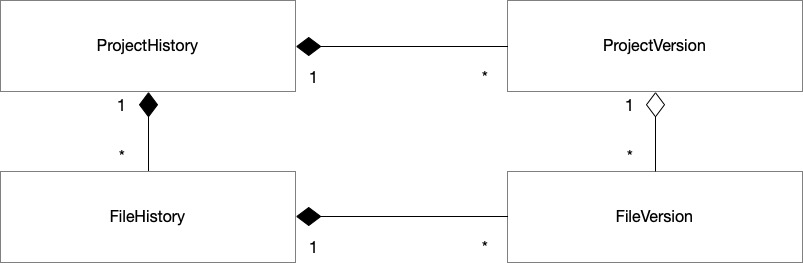
\includegraphics[width=0.6\textwidth]{images/approach/EvolutionModel.jpg}
    \end{center}
    \caption{Evolutionary Model}
    \label{fig:EvolutionaryModel}
\end{figure}


To model the evolution of software systems, we developed the model 
shown in \autoref{fig:EvolutionaryModel}. It is based on Hismo by Tudor Girba \cite{Girba2005}.
The need to develop a novel evolutionary model comes from the fact that Hismo was designed to work with another versioning system: Subversion (SVN). 
These are the four main concepts of our model: 
\begin{itemize}
    \item \textbf{ProjectHistory}: represents the history of a repository. It holds two sets: a set of FileHistories and ProjectVersions. 
    \item \textbf{FileHistory}: represents a repository file. We consider each file as an entity of the system. Even if the entity's name or location is changed, our mode will treat it as the same. So, our approach is resilient to a renaming and moving activities. Each FileHistory holds a set of FileVersions, each representing a different version of the entity at a particular time.  
    \item \textbf{ProjectVersion}: represents a commit or a version of the system. 
    For each changed file inside a commit, the respective ProjectVersion contains a FileVersion representing that change.
    A ProjectVersion holds contextual information about the commit, such as the timestamp, the hash of the commit, and its message.
    \item \textbf{FileVersion}: represents the version of a file at a particular point in time.
    It is responsible for holding all the evolutionary information of an entity. 
\end{itemize}

One of our goals was the possibility of analyzing a large repository in an acceptable amount of time. 
In other words, our approach needs to be scalable. We present a scalable approach based on the concept of partial history.
A partial history holds information about a specific range of time of the ProjectHistory. 
It can be seen as a subset of a ProjectHistory. 
We can split the repository's history into multiple parts, each represented by a partial record. Then when all the analyses are completed, we merge them to reconstruct the whole story of the repository.

Software systems are hard to understand due to the complexity and the sheer size of the data to be analyzed.
In our approach, we aim to make an interactive 3D representation to ease the comprehension task of a developer. 
To visualize a project, we introduce the concept of \textbf{view}. We define a view as a way to illustrate the evolution of a project given a set of specifications. This set of specifications determines how the view must be built. For example, if we want to traverse the repository history by year, this information is part of the specification. A view holds a set of frames, called \textbf{AnimationFrame}, each representing the repository's state at a specific moment of its evolution. Therefore, the entire history of the repository is displayed by rendering these AnimationFrames consecutively, like in a movie. 
We provide two visualization strategies to group commits into AnimationFrames: by timestamp and by commit. Both of them traverse the whole history from the beginning until the end.
Only the most recent one is considered when an AnimationFrame is created, and multiple commits were made on a file. 
To represent the system's state, an AnimationFrame holds a set of \textbf{ViewFigures}, each representing a system file, that uses the following visual concepts: 
\begin{itemize}
	\item \textbf{position}: to describe the ViewFigure's location in the 3D environment. We adopted a spiral layout with an outward direction. Older entities are positioned at the center of this spiral, whereas newer entities are always close to borders.
	\item \textbf{color}: to describe the last action made on a file. The user can customize the mapping. 
	\item \textbf{age}: to represent the amount of time elapsed between the last action made on a file and the currently displayed AnimationFrame.
	\item \textbf{shape} and \textbf{opacity}: to distinguish between the different types of files (e.g. we can represent Java files with boxes and binary files with hemispheres). 
	\item \textbf{height}: to represent the value of a metric previously selected by the user. 
\end{itemize}

Displaying lots of information on the screen might not be an efficient way to gather crucial aspects of the evolution of a software system. We want to play AnimationFrames sequentially, like in a movie. Therefore, users might not have the time to understand the differences between the current and the previously displayed AnimationFrame. To overcome this issue, we provide an auditorial representation of an AnimationFrame to support understanding its changes. The goal is to support the sight sense, combining it with hearing, by playing audio notes that are recognizable by the user, generated from similar but complementary information, to understand an AnimationFrame better. 

Generated sound melodies depend upon the value of a pre-selected metric. For example, we can create a new metric to play how many Java files were added. In our approach, we assign distinct sounds to each of the metrics, e.g., the number of commits will influence the tempo of our melody (BPM) and will be represented by a sound similar to a heartbeat.

The output of this approach is a piece of music representing a system's evolution. It is composed of several different sounds equal to the number of metrics used in its generation. The idea is to use these values to control BPM, pitch, and the amplitude of a note. 

Therefore we designed and implemented SYN, a tool that supports the software evolution comprehension approach. 
It is composed of a set of modules, as follows:
\begin{itemize}
    \item \textbf{Core}: it holds classes representing basic SYN concepts such as ProjectHistories, ProjectVersions, and FileVersions. It also provides abstract classes, open to any implementation, to achieve the extensibility goal and it implements the auralization approach.
    \item \textbf{CLI}: provides a Command Line Interface (CLI) to users.
    \item \textbf{Analyzer}: implements our scalable analysis. 
    \item \textbf{Server}: provides GraphQL endpoints to retrieve data and display them in a user interface. 
    \item \textbf{Visual Inspector}: shown in \autoref{fig:SYNVisual} used to debug and visually depict information collected during the analysis. It is composed of four parts
In box \encircle{A}, a 3D environment displays FileHistories on a virtual plane. The camera is not fixed, and the view angle and the zoom level can be controlled with the mouse. 
In box \encircle{B}, we have a card with general information about the project visualization. 
This card includes the project's name, the animation number, the dates of the animation frame, and its commit list. The slider shows the overall progress of the display, two buttons to jump to the subsequent or previous animation, and finally, one button to jump to the following animation with the time interval previously set. 
All the preferences specified during the project setup can be changed by clicking on the three dots in the top right corner.
In box \encircle{C}, we have a card to inform the user of the number of entities the UI renders. 
And finally, box \encircle{D} appears when an entity is selected with the mouse. 
\end{itemize}

The visual inspector is a helpful tool to understand and debug the analysis process of SYN. However, it has performance issues in rendering large systems. The main problem stems browser environment as it has limited resources. We experienced a significant frame rate drop when rendering large systems. To overcome this limitation and prove the versatility of our approach, we rendered large systems with POV-Ray, \footnote{\url{http://www.povray.org}} an open-source tool for creating high-quality three-dimensional graphics. We developed an extension of SYN that, given a View, produces a \texttt{pov} file for each AnimationFrame, following the same approach adopted in the visual inspector.  



\begin{figure}
    \center
    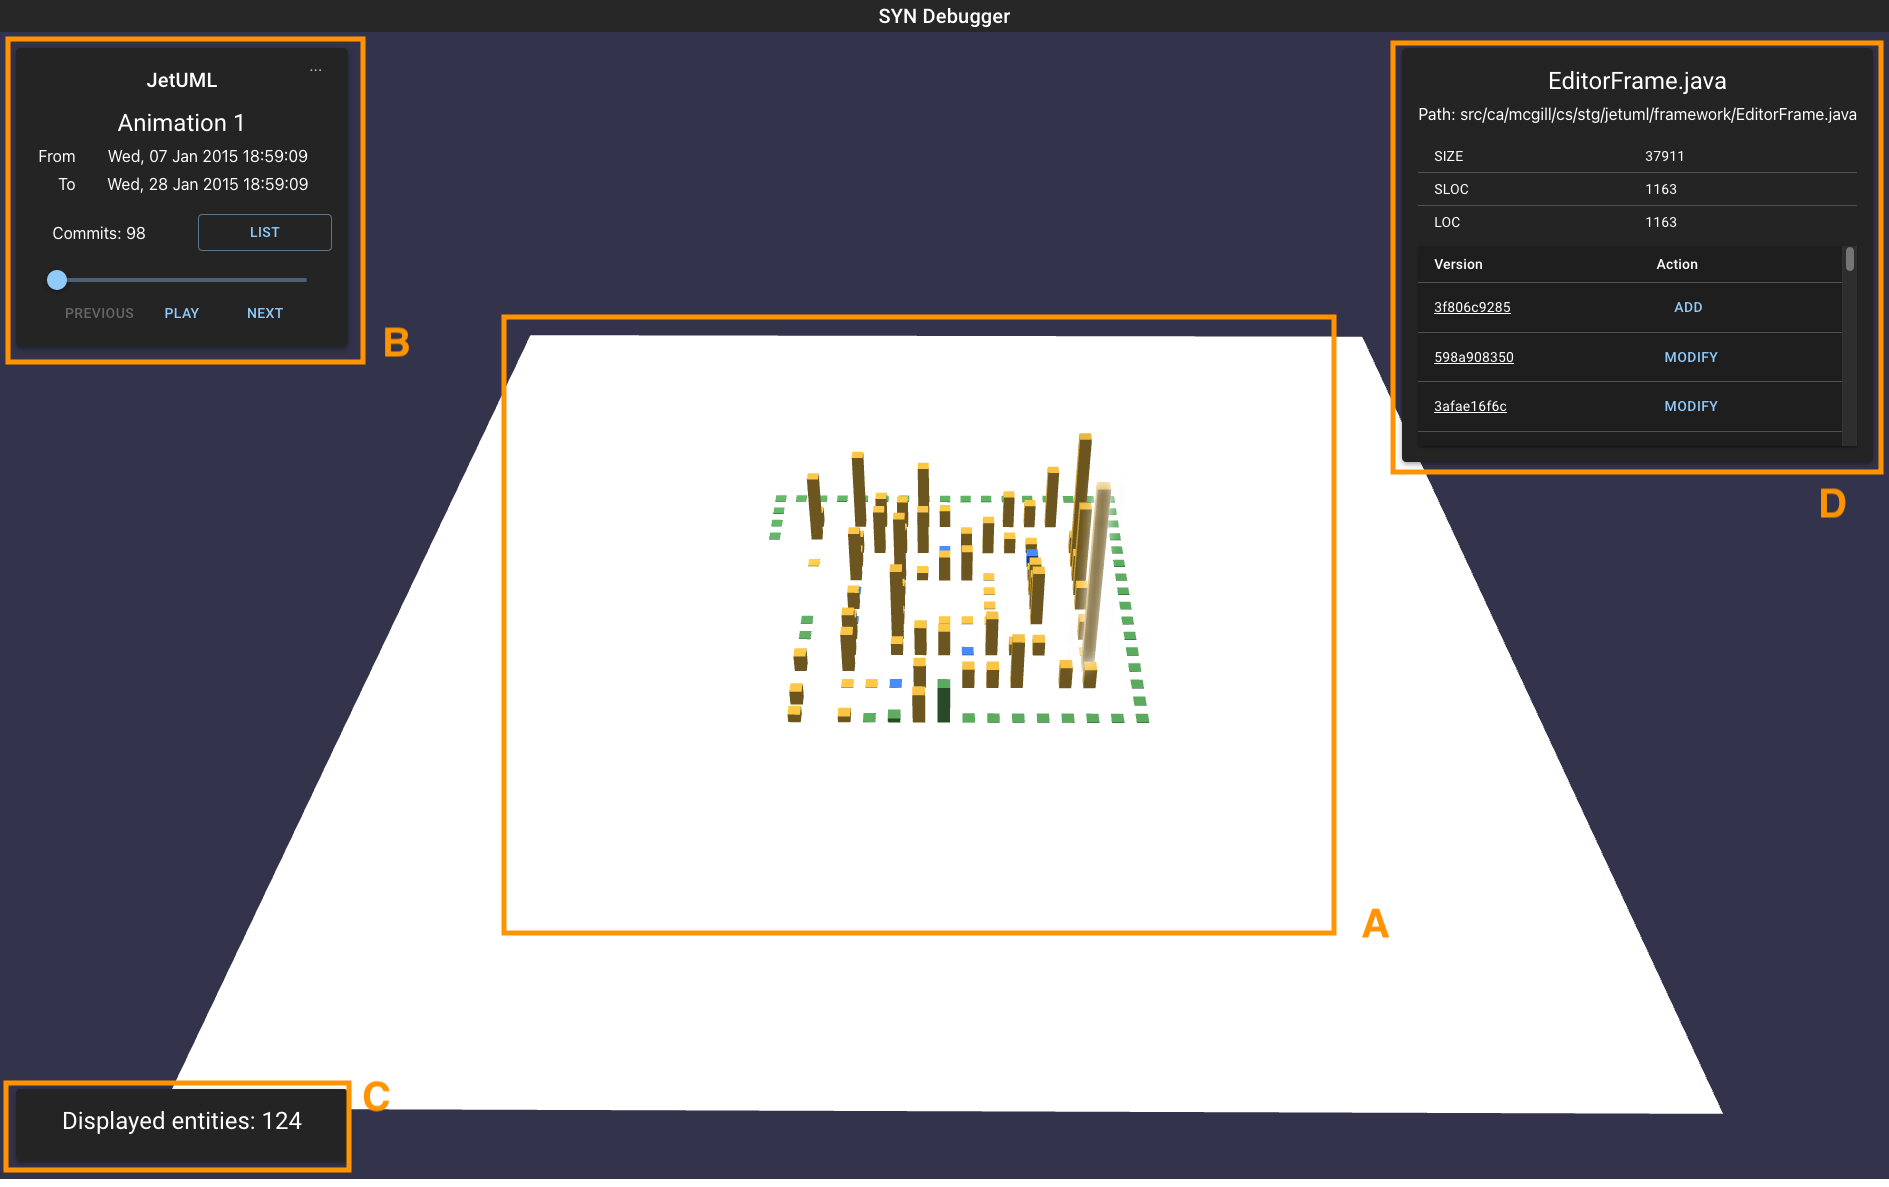
\includegraphics[width=\textwidth]{images/implementation/SYNUI-fileHistory.png}
    \caption{SYN Visual Inspector}
    \label{fig:SYNVisual}
\end{figure}

\section*{Case studies}
\graphicspath{ {images/casestudies} }

\begin{figure}[ht]
    \begin{subfigure}{0.48\textwidth}
        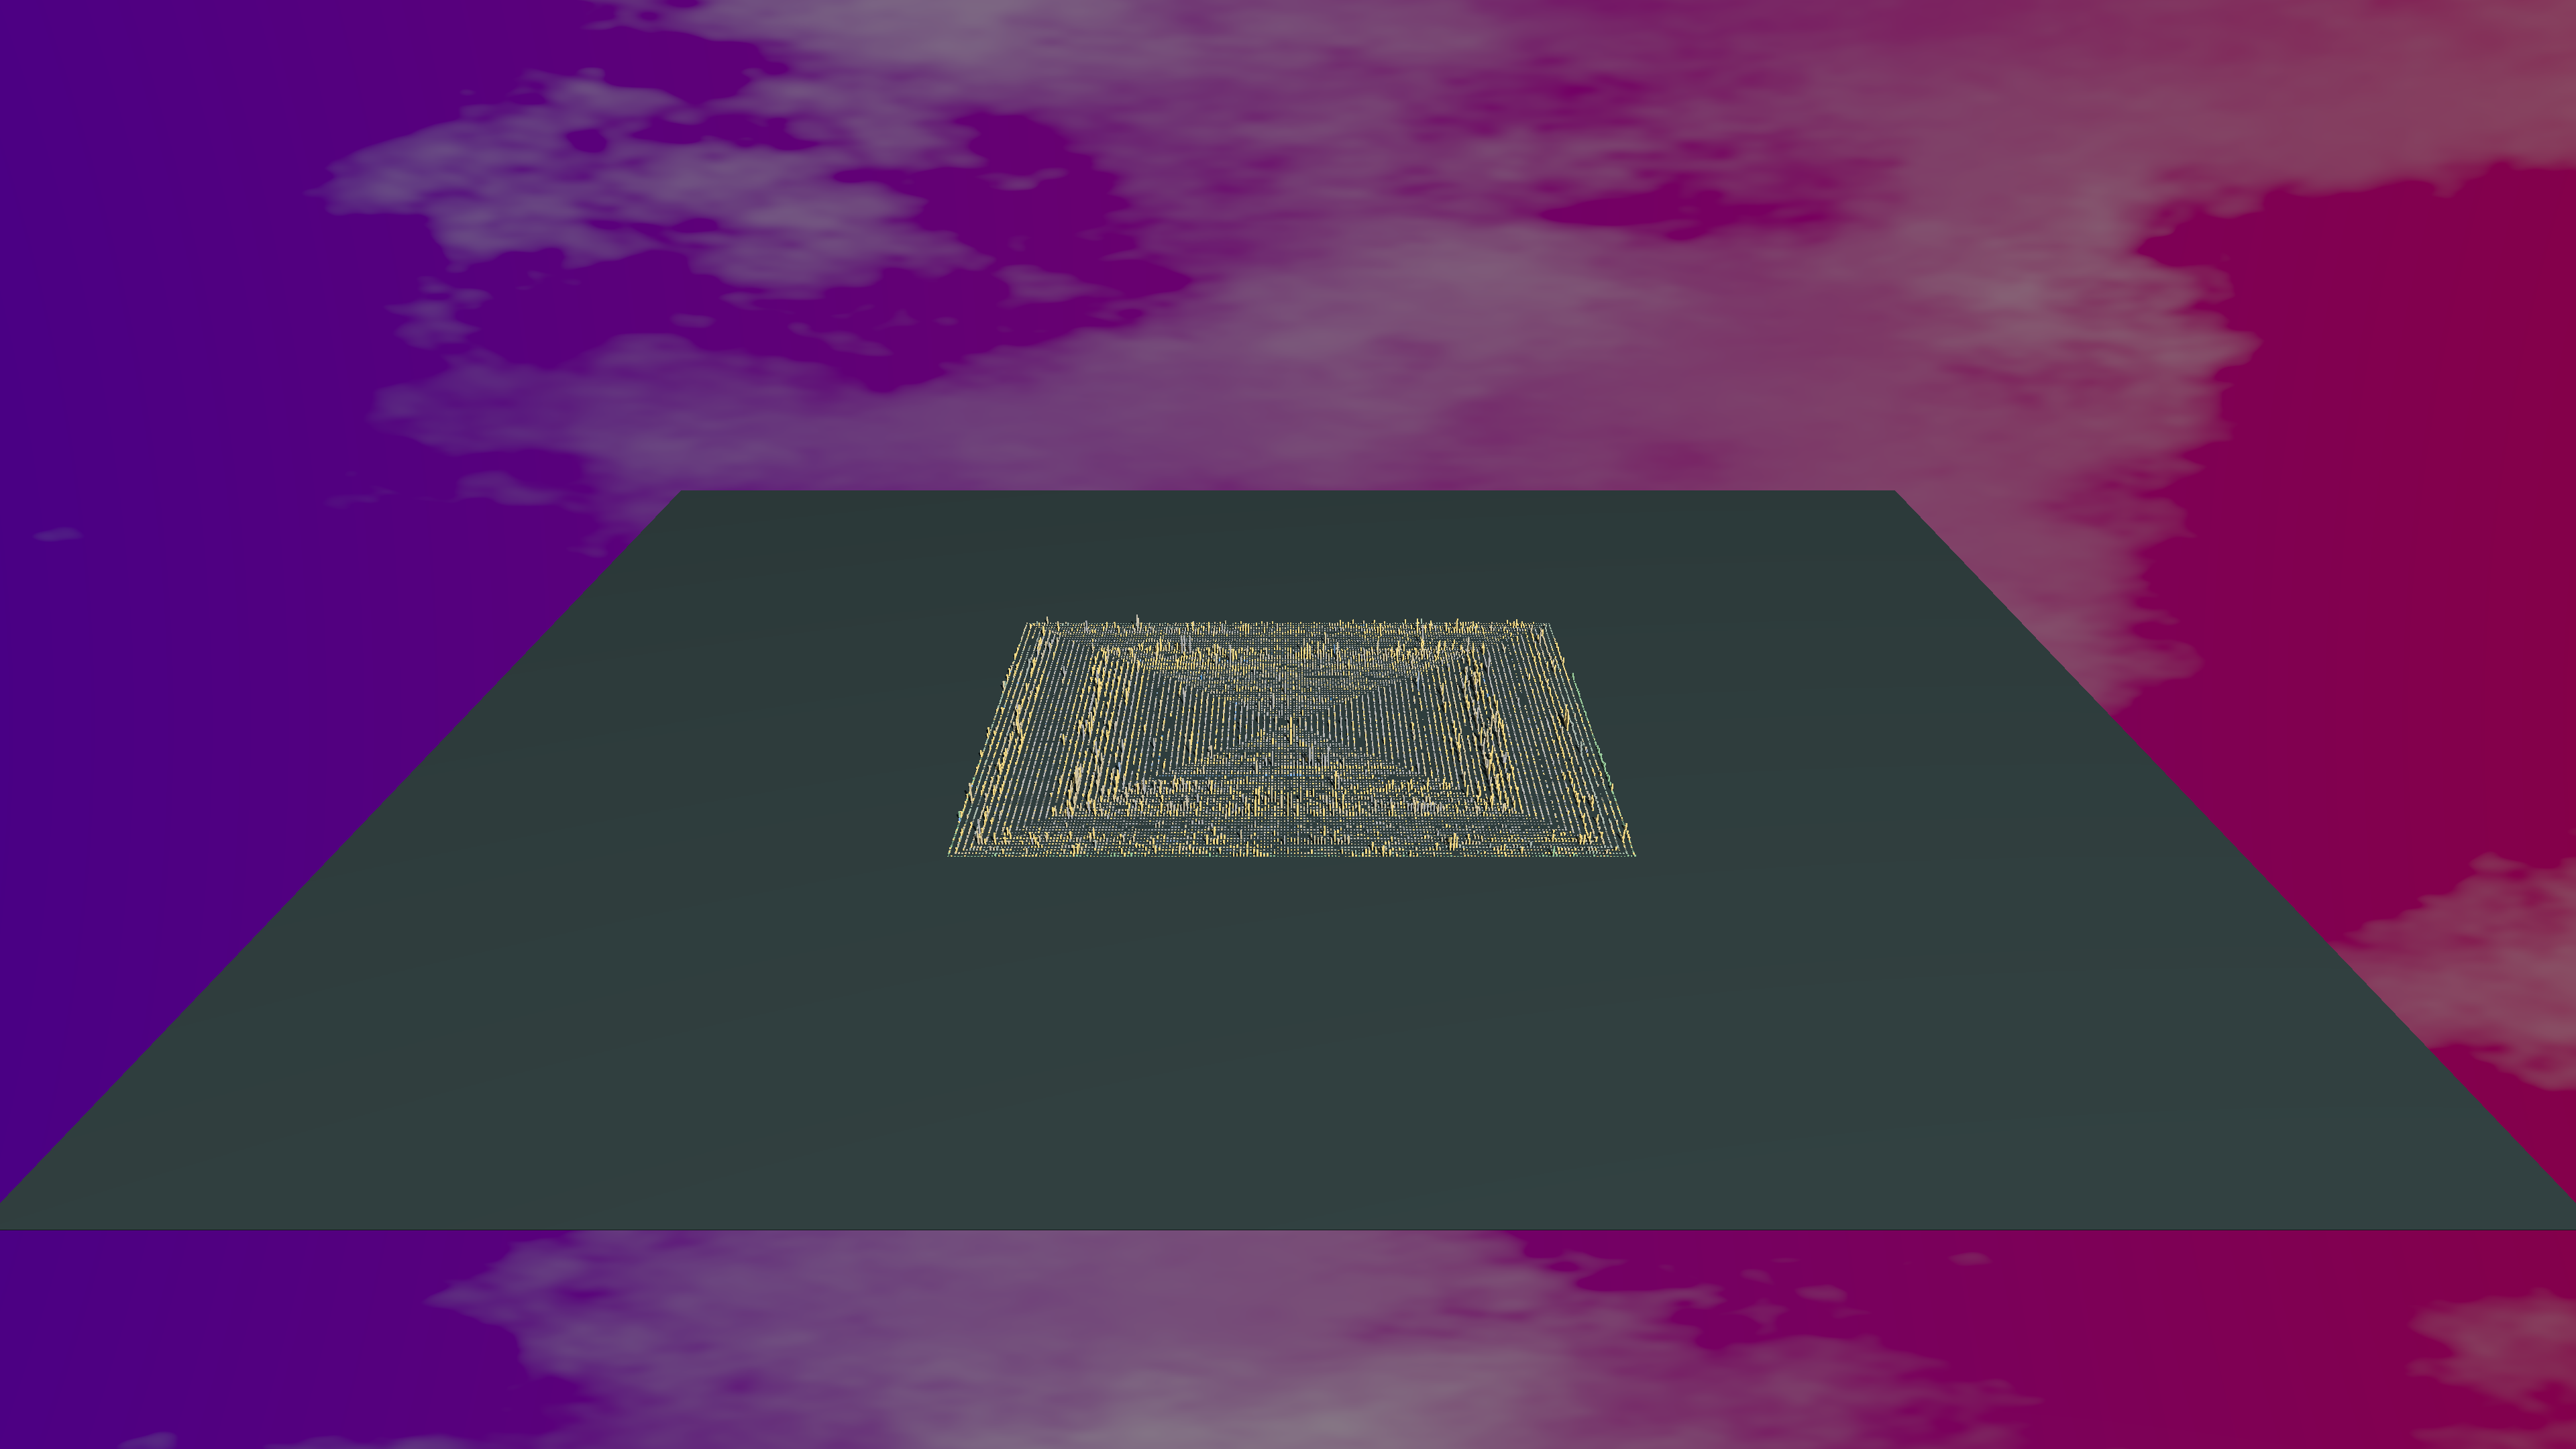
\includegraphics[width=\linewidth]{Linux/Animation001.png}
        \caption{Linux in April 2006 (1 year)} 
        \label{fig:Linux_V7_S1}
    \end{subfigure}\hspace*{\fill}
    \begin{subfigure}{0.48\textwidth}
        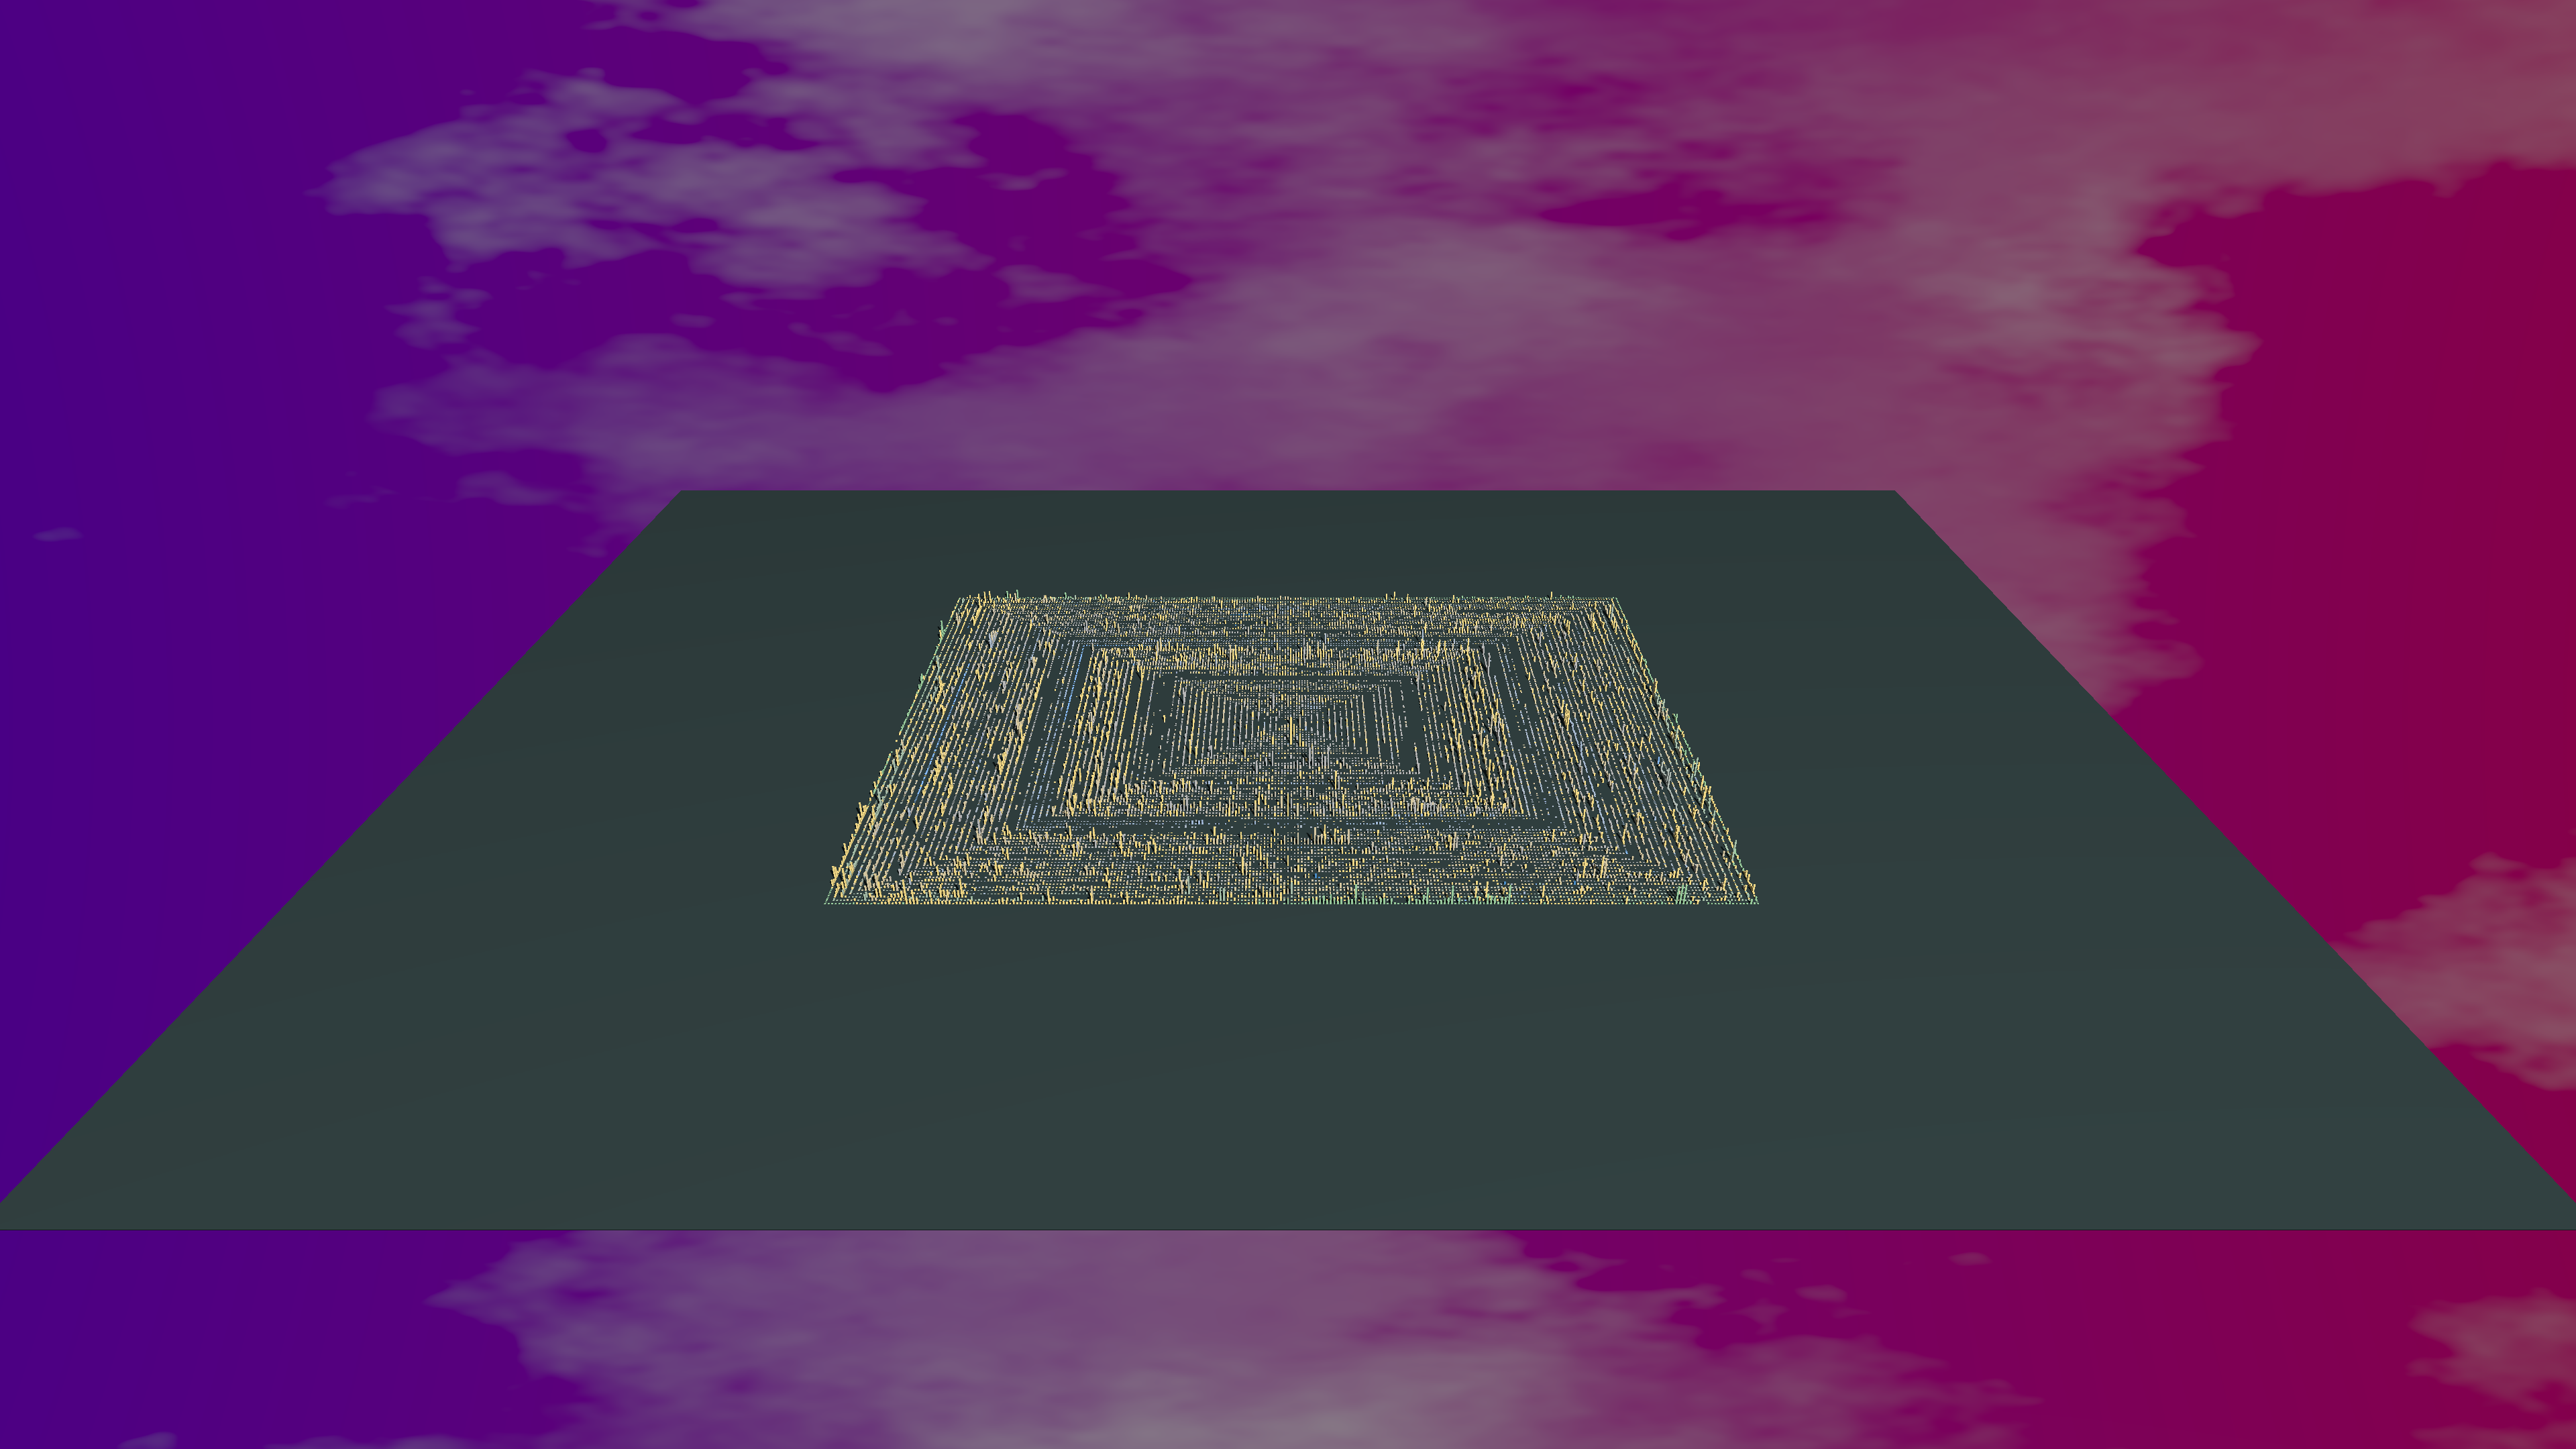
\includegraphics[width=\linewidth]{Linux/Animation004.png}
        \caption{Linux in April 2009 (4 year)} 
        \label{fig:Linux_V7_S2}
    \end{subfigure}
    \medskip
    \begin{subfigure}{0.48\textwidth}
        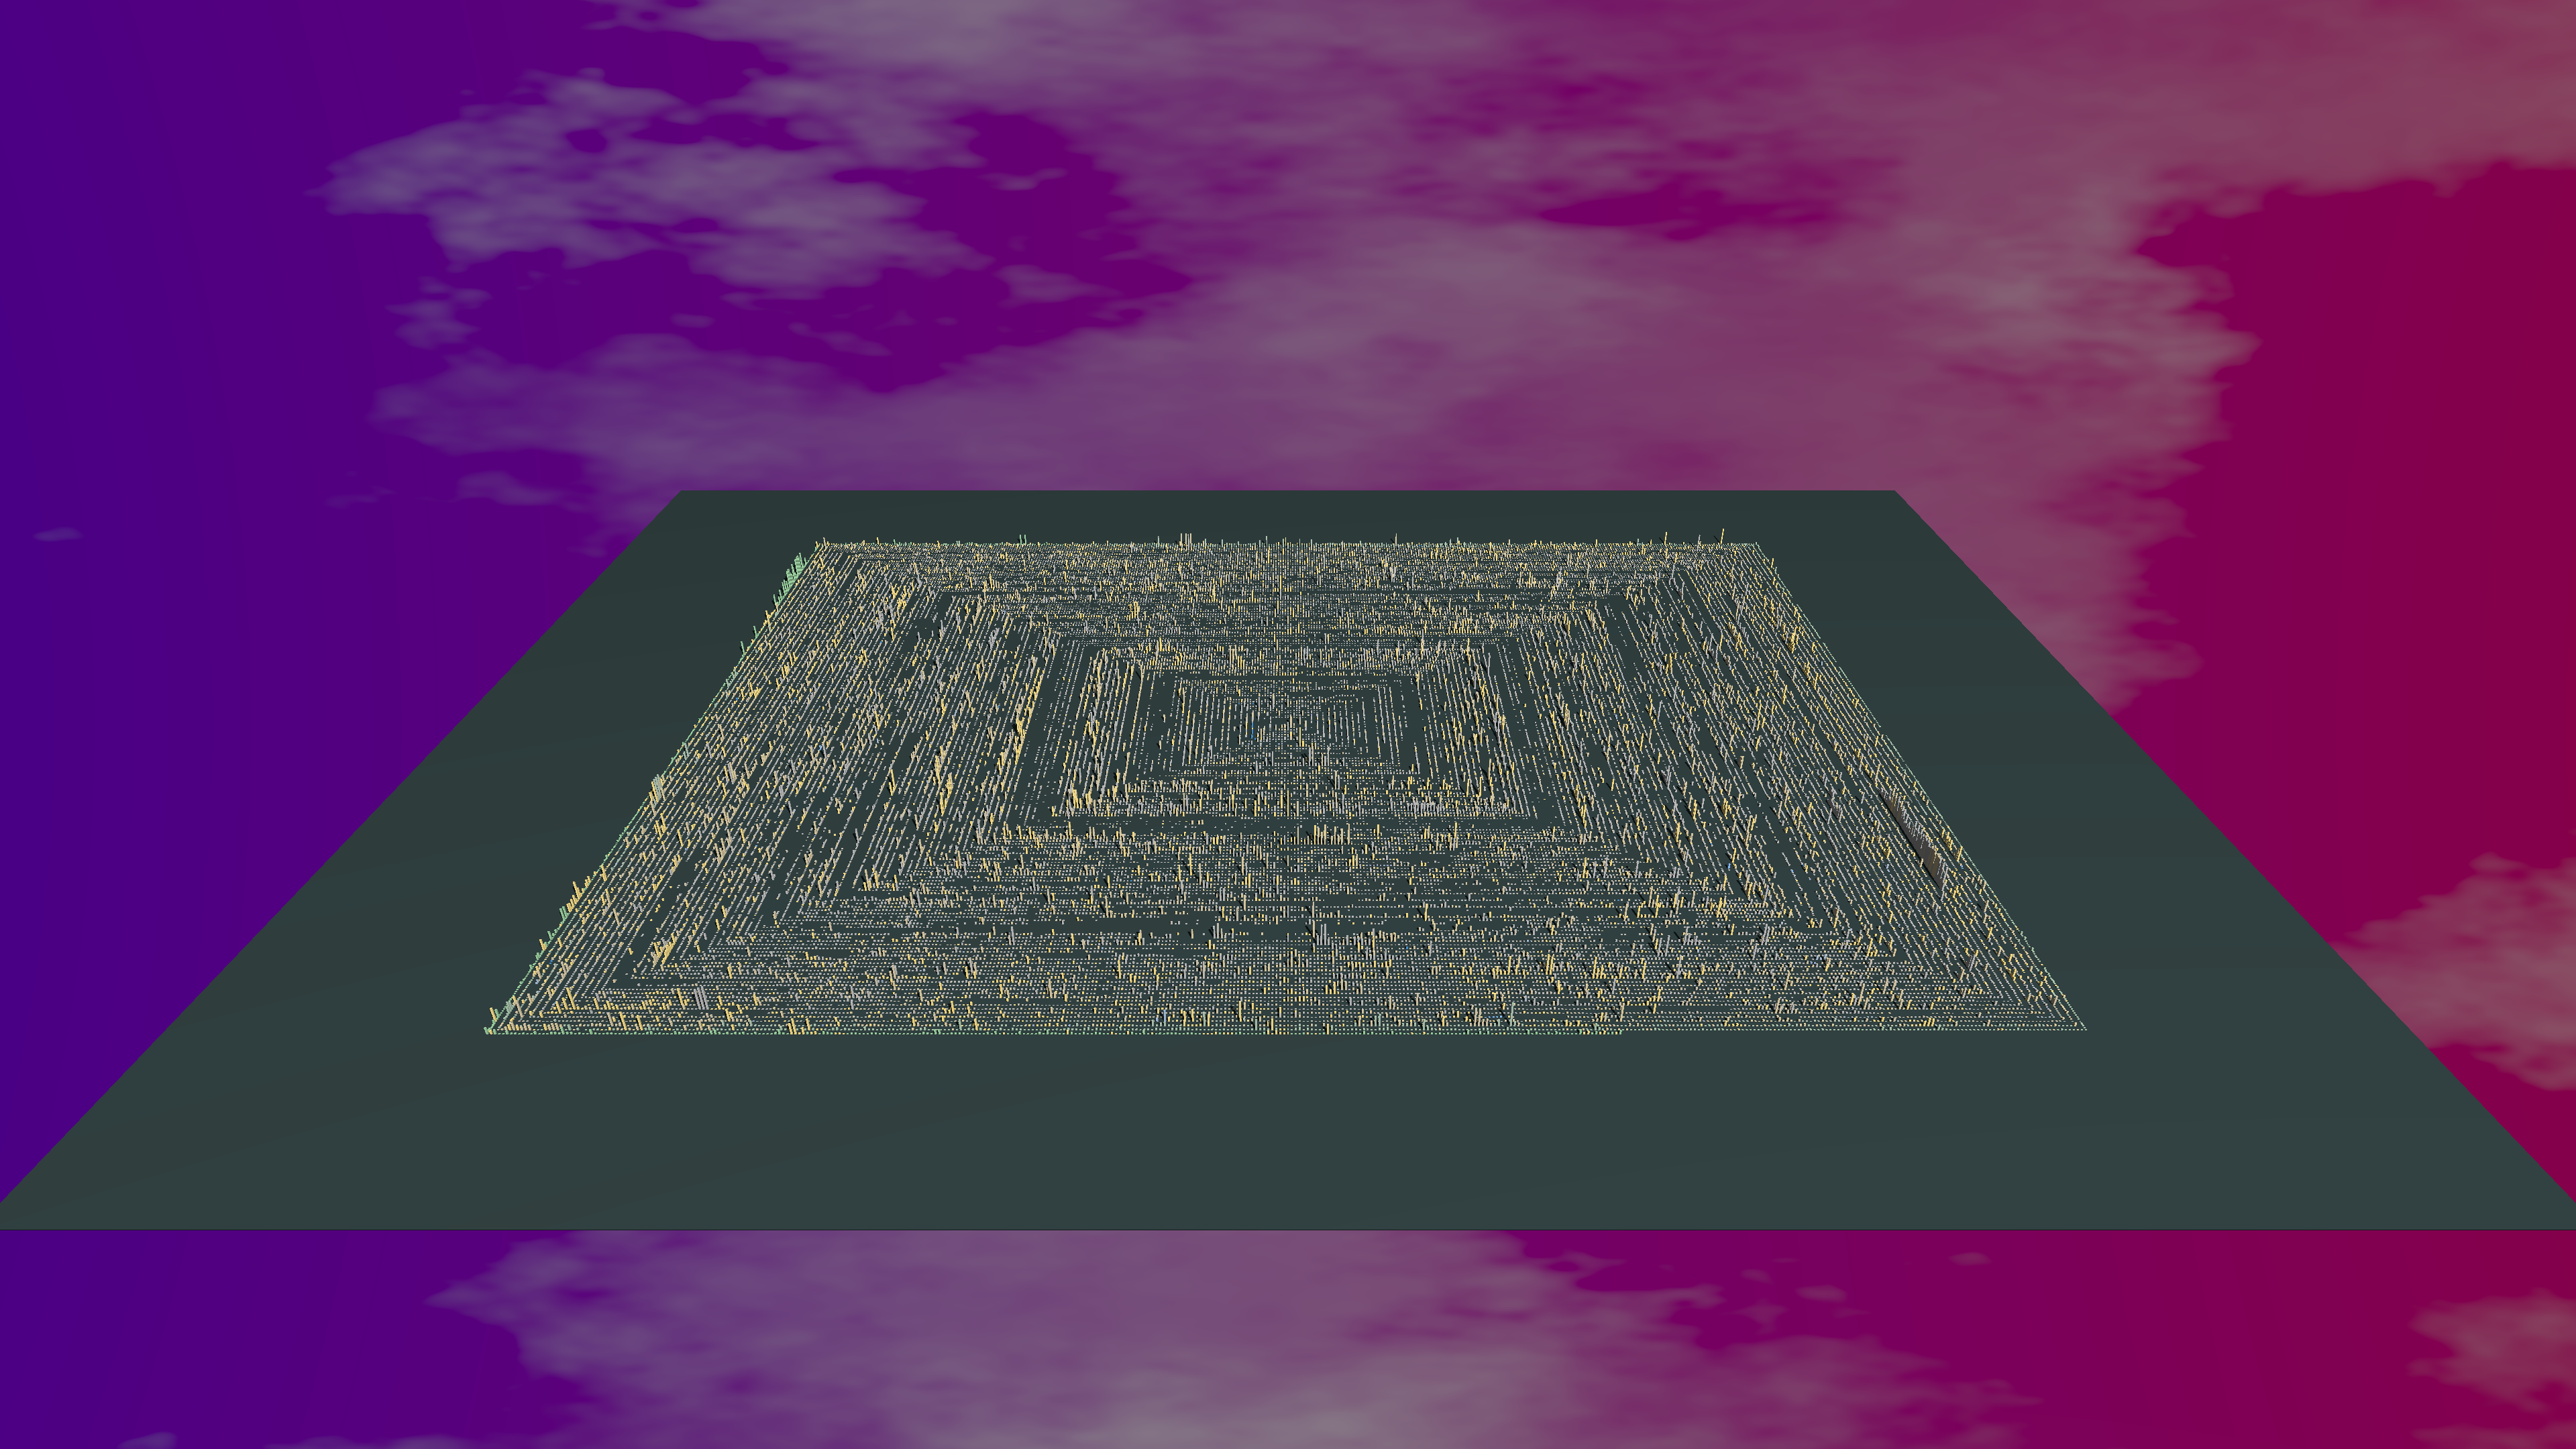
\includegraphics[width=\linewidth]{Linux/Animation012.png}
        \caption{Linux in April 2017 (12 year)} 
        \label{fig:Linux_V7_S3}
    \end{subfigure}\hspace*{\fill}
    \begin{subfigure}{0.48\textwidth}
        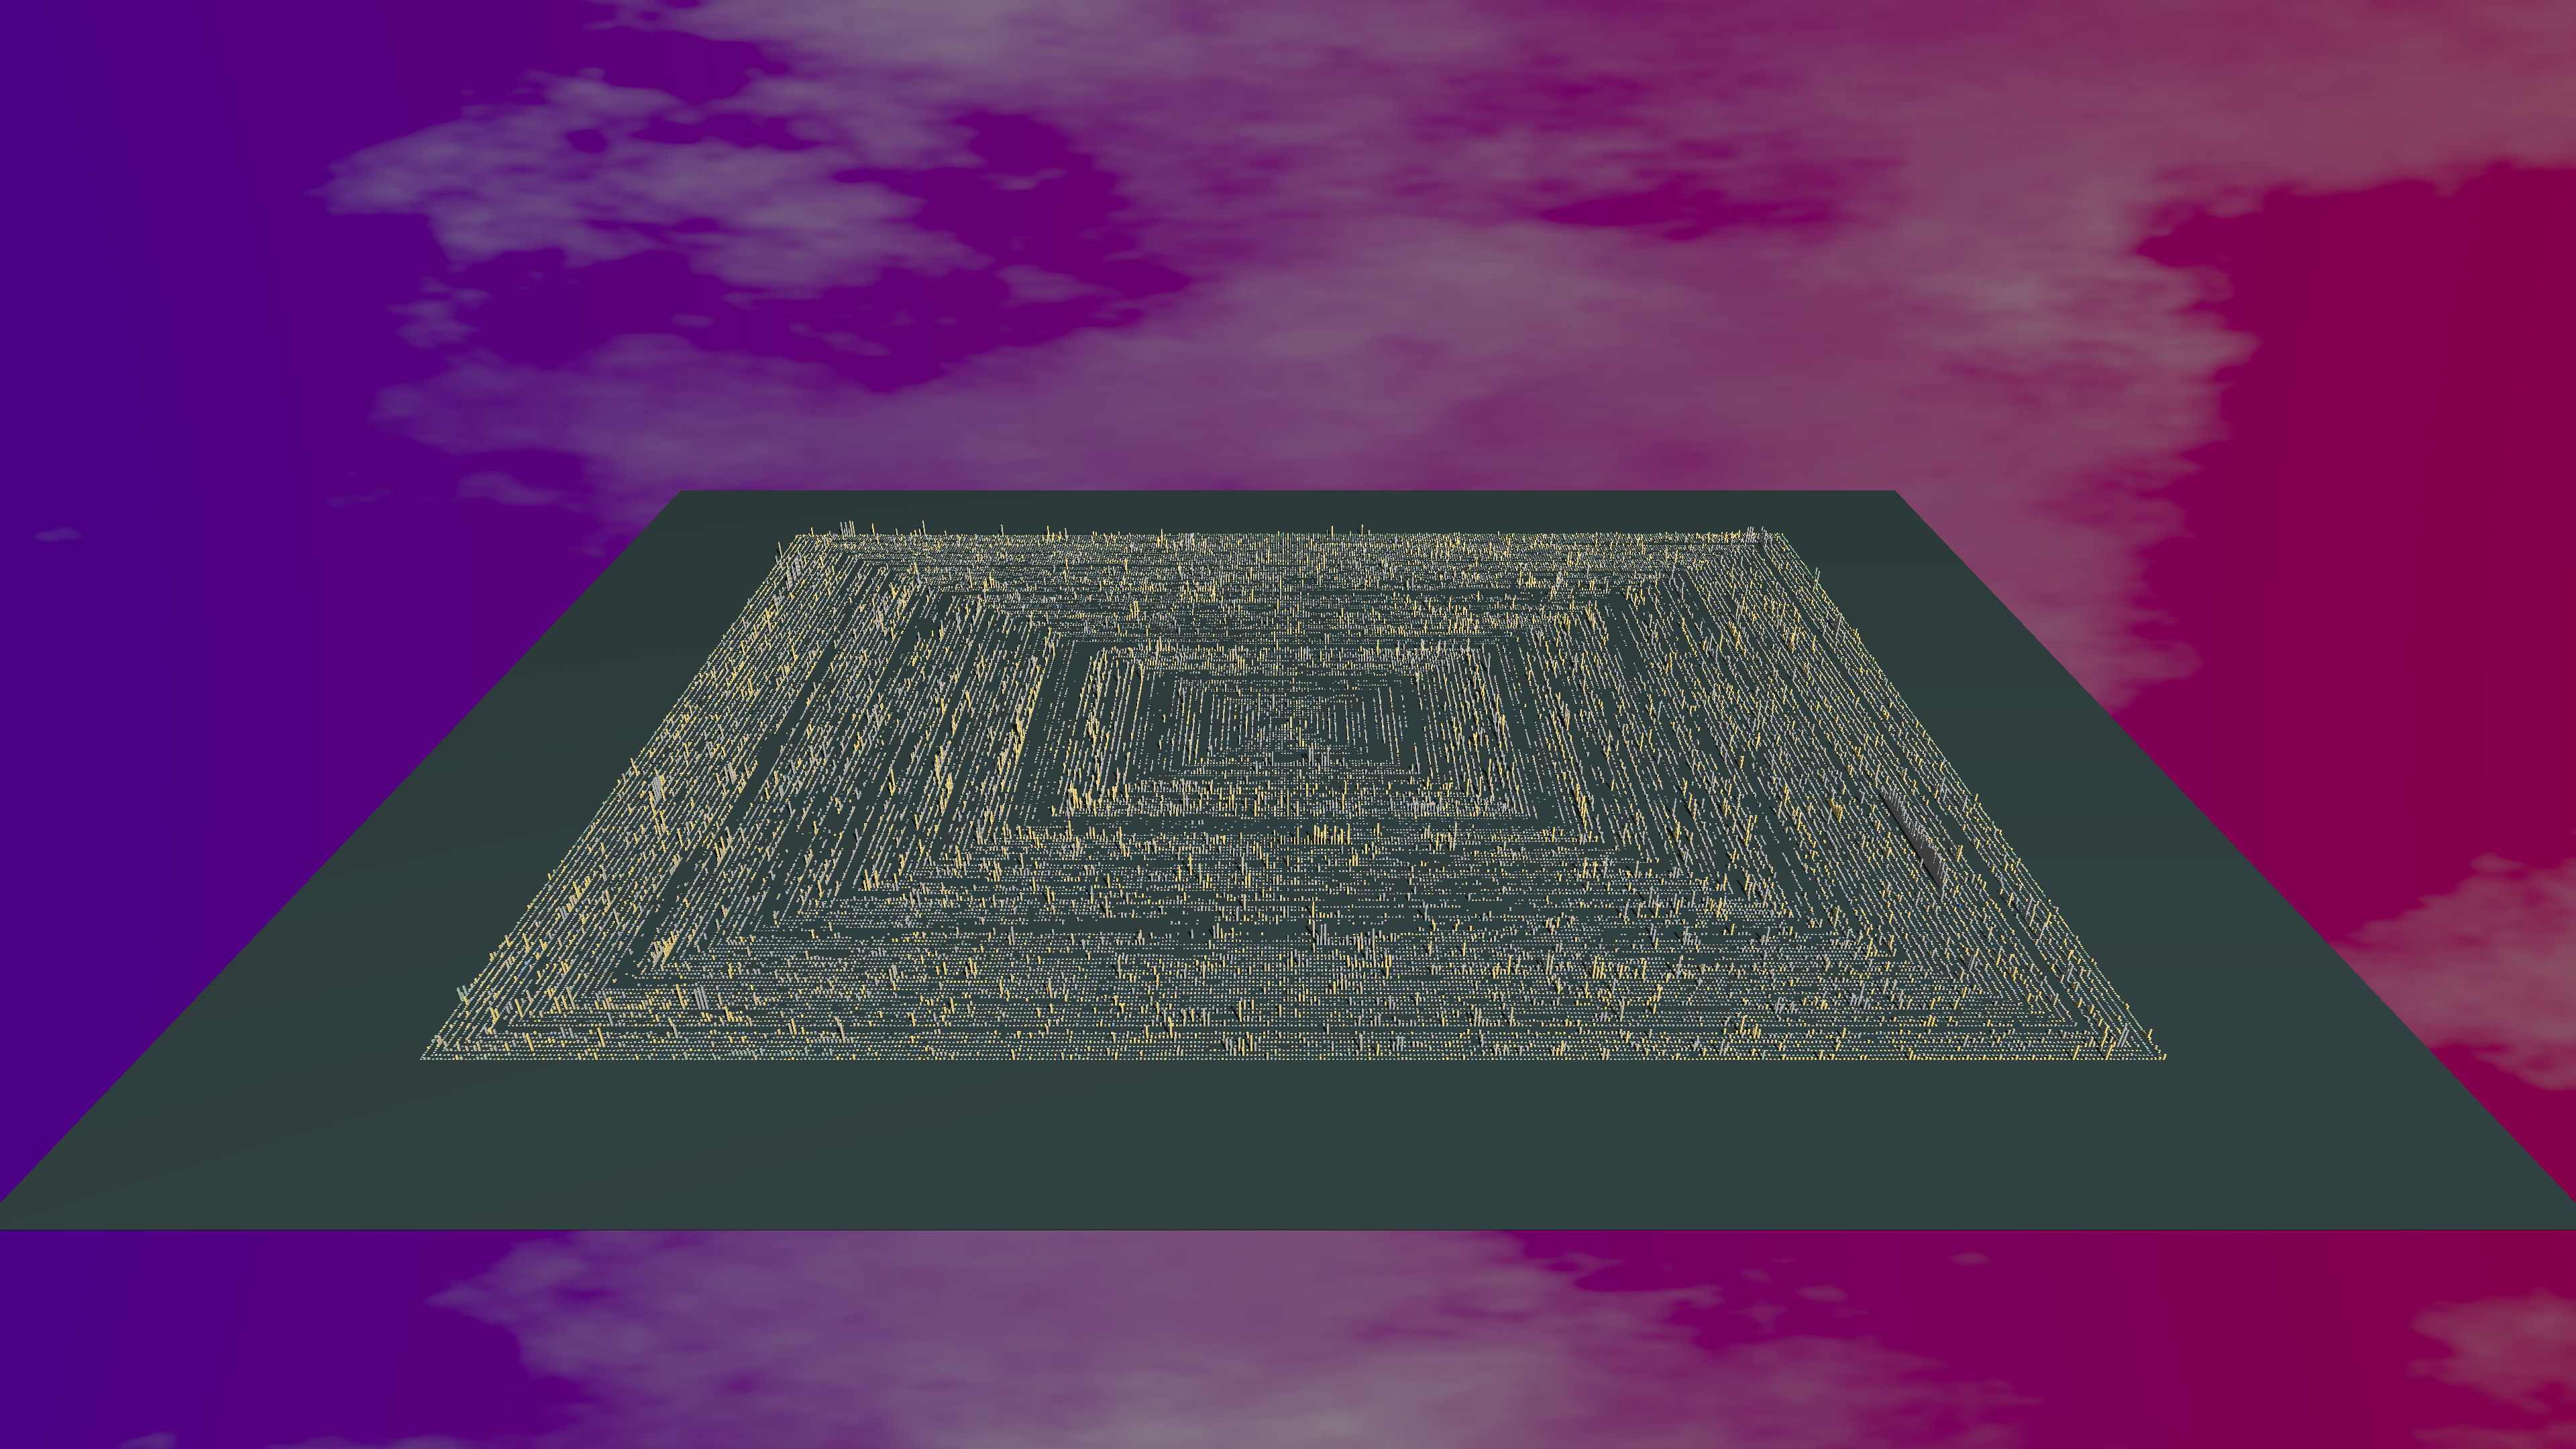
\includegraphics[width=\linewidth]{Linux/Animation014.png}
        \caption{Linux in April 2019  (14 year)} 
        \label{fig:Linux_V7_S4}
    \end{subfigure}
    \medskip
    \begin{subfigure}{0.48\textwidth}
        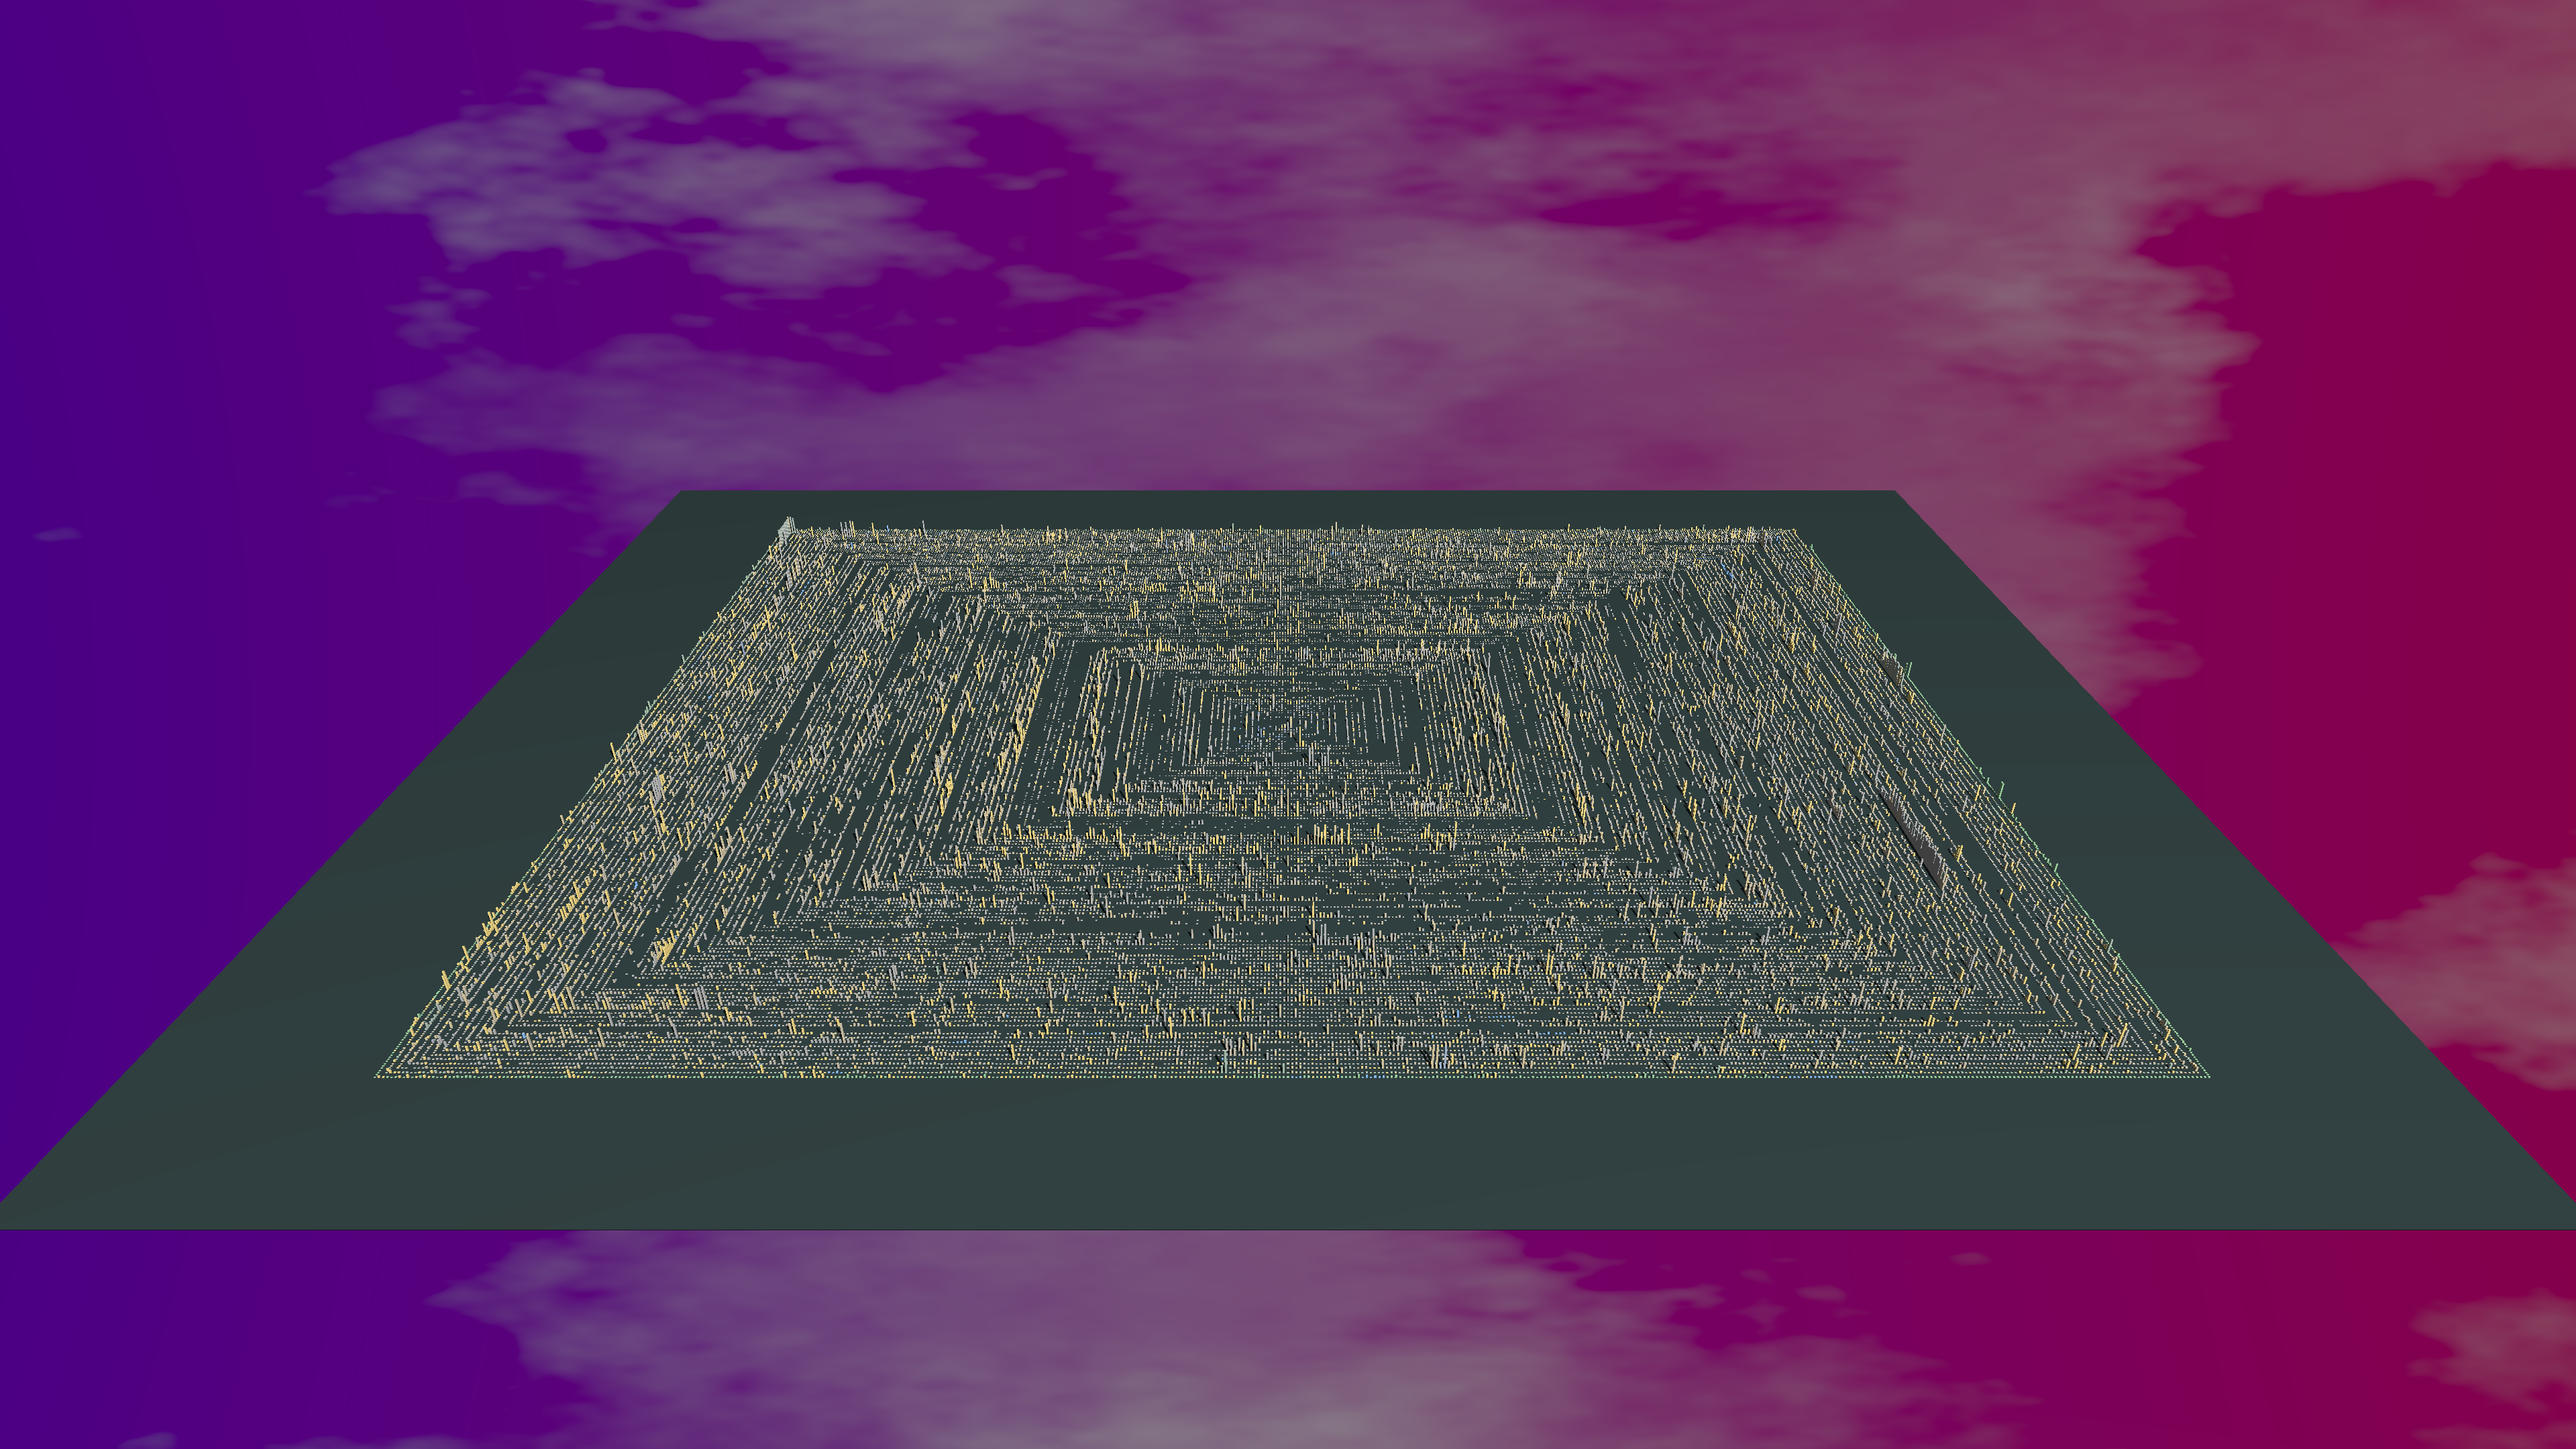
\includegraphics[width=\linewidth]{Linux/Animation015.png}
        \caption{Linux in April 2020 (15 year)} 
        \label{fig:Linux_V7_S5}
    \end{subfigure}\hspace*{\fill}
    \begin{subfigure}{0.48\textwidth}
        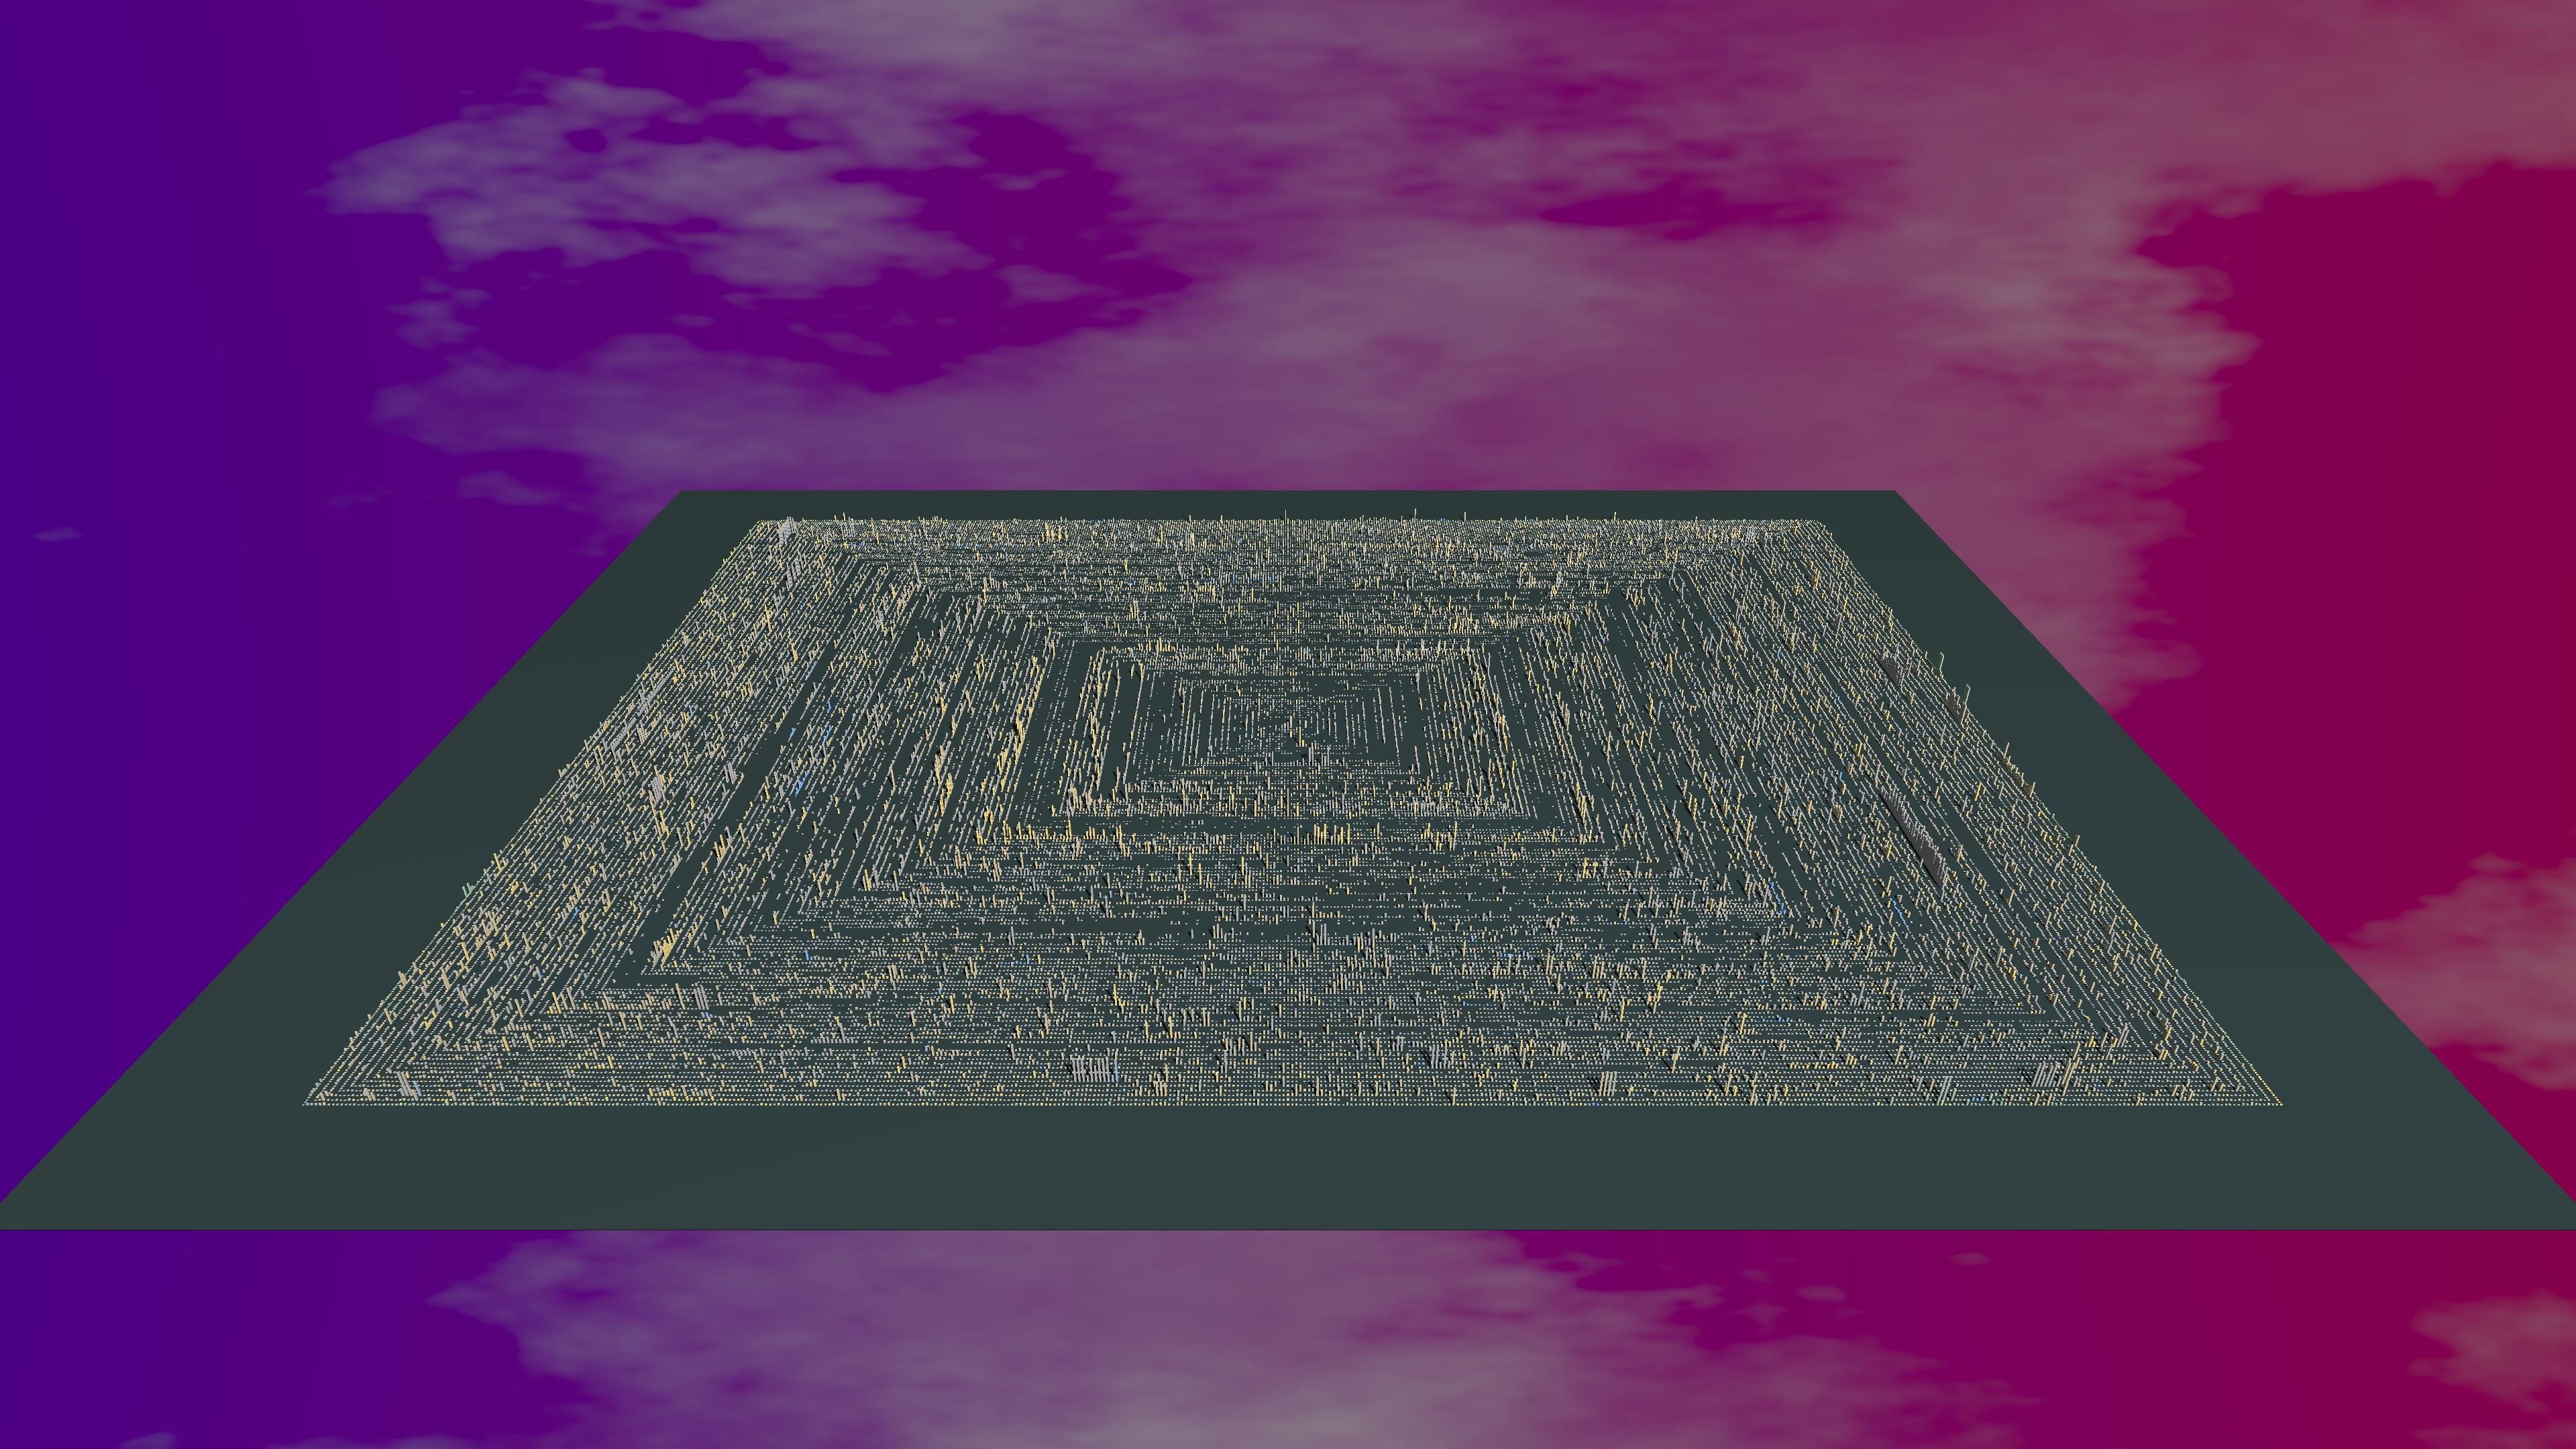
\includegraphics[width=\linewidth]{Linux/Animation017.png}
        \caption{Linux in April 2022 (17 year)} 
        \label{fig:Linux_V7_S6}
    \end{subfigure}
    
    \caption{Linux evolution} 
    \label{fig:Linux_V7}
\end{figure}

We applied SYN to real-life systems and presented several insights and reflections. For example, in \autoref{fig:Linux_V7}, taken from the Linux case study, we saw how the codebase of Linux evolved since its move to git. The development activity was constant throughout these 17 years. The codebase started with 19,705 files and reached 77,183 in April 2022, almost four times its original size. During this time, they evolved the kernel to develop new features and slowly started a process to remove the files that were added 17 years ago. As we can see, the center of the spiral began to become sparse. Nonetheless, it still holds many files, which means that the current version of Linux relies on files written more than 17 years ago.
We combined our visualization and auralization approach in a video depicting the evolution of Linux available at \url{https://workInProgress.com}. 


\section*{Conclusions}

In the thesis, we presented an approach to mine, visualize and auralize large software repositories. The goal of this thesis was to explore new solutions to represent evolution. We cover all the stages required to reconstruct the history of a git repository, from the historical collection of information to the graphical data representation and visualization. We developed it with an agnostic approach against the programming language. Therefore, an extension of the system is needed to collect and visualize specific kinds of information. Our contributions can be summarized as follows:
\begin{enumerate}
    \item \textbf{The mining and modeling of a large git repository's history}. We present an approach to rebuilding the history of a git repository by traversing the repository's history. It starts from the first commit and analyzes all the subsequent commits until the end.
    We extract information about the modified files for each commit, parse it, and finally serialize it in a file on the local storage. The root element of our model is the history of a project that holds a set of files. An action recorded by a commit made on a file is also represented.
    \item \textbf{The sensorial software evolution visualization}. It exploits synesthesia, the production of a sense impression relating to one sense by stimulating another. It represents the evolutionary process through an interactive visual depiction of evolving software artifacts. It enables the comprehension of both the structural and the evolutionary prospectives. Moreover, SYN, the tool that implemented this approach, allows the user to customize visualization properties deeply. This approach provides the following benefits:
    \item \textbf{Auditive portrayal of the evolution}. It consists of a guideline suggesting how to compose audio sounds representing the evolution of a project. The proposed methodology was tested with two systems and presented with the JetUML and Linux case study analysis. The main benefit provided by this approach is the support of the visualization. It provides additional information without displaying them. Consequently, the listener can infer additional aspects of the analysis.
\end{enumerate}   
%%%%%%%%%%%%%%%%%%%%%%%%%%%%%%%%%%%%%%%%%%%%%%%%%%%%%%%%%%%%%%%%%
%%%	BIBLIOGRAPHY %%%%%%%%%%%%%%%%%%%%%%%%%%%%%%%%%%%%%%%%%%%%%%%%
%%%%%%%%%%%%%%%%%%%%%%%%%%%%%%%%%%%%%%%%%%%%%%%%%%%%%%%%%%%%%%%%%

\newpage
\bibliographystyle{abbrv}
\bibliography{biblio}

\end{document}